In this chapter we present comparisons between seismic hazard results computed using OpenQuake and alternative software for real national/regional scale seismic hazard models. We present three cases: the seismic hazard model for the 2005 national building code of Canada (\cite{adams2003}, \cite{halchuk2008}), the 2008 U.S. national seismic hazard model (\cite{petersen2008}), and the 2012 national seismic hazard model for Australia (\cite{burbidge2012}). We refer the reader to the original reports for an in-depth description of each model. Here we present only the main features and the aspects of interest for the software implementation.


\section{The national seismic hazard model for the 2005 building code of Canada}

\subsection{The seismic source model}
To capture epistemic uncertainties in the seismic source definition, two complete seismic source models are defined: the historical (\textbf{H}) and regional (\textbf{R}) models. The historical model uses relatively small source zones drawn around historical seismicity clusters, while the regional model defines larger, regional zones reflecting seismotectonic units. Both models are composed of area sources, with the only exception of the Queen Charlotte fault (in western Canada) treated as a fault source. Occurrence rates in each source are defined through a double-truncated Gutenberg-Richter distribution, with minimum magnitude equal to 4.75.
Epistemic uncertainties in the magnitude-frequency distribution are captured by the definition for each source of three possible ($a_{GR}$, $b_{GR}$) pairs and three possible maximum magnitudes. Each source is also associated to three possible hypocentral depths. The model prescribes also a floor model (\textbf{F}) for the relatively aseismic central part of Canada and a deterministic model for the Cascadia subdution zone (\textbf{C}).\\
Earthquake ruptures associated with area sources are assumed to have no spatial extension (that is point ruptures), while earthquakes on faults follow a magnitude-length scaling relationship ($L=10^{-1.085 + 0.389 m}$)

\subsection{The ground motion model}
The ground motion model distinguishes between eastern and western Canada because of the different properties in the crust. For eastern and central Canada the GMPE model of \cite{ab1995} is used. For western Canada the model of \cite{bjf1993} is used for shallow crustal sources, while for deep intraslab sources the model of \cite{y1997} is adopted. Epistemic uncertainties are included by defining, for each GMPE, a pair of parallel alternative relations, with higher and lower mean values.

\subsection{Reference site conditions}
Hazard maps are computed for a \textit{reference} ground condition corresponding to "Site Class C" (firm-ground), defined by a 360 to 750 m/s $Vs_{30}$. For central and eastern Canada, hazard map values computed with the hard-rock GMPE of \cite{ab1995} are adjusted for firm-ground. That is, seismic hazard spectral values are amplified by a period-dependent 'reference ground condition' factor (see Table 2 in \cite{adams2003}). For western canada, the model of \cite{y1997} is adjusted for firm-ground. The model of \cite{bjf1993} does not require instead any adjustment given that its "Soil Class B" is identical to "Site Class C".

\subsection{Implementation of the model in the OpenQuake-engine}
Currently, only the \textbf{H} and \textbf{R} models are implemented in the OpenQuake-engine. We set the discretization step for area sources to 5 km, and model ruptures as points. The discretization step for the Queen Charlotte fault is instead 2 km, and the rupture extension is modeled using the magnitude-area scaling relationship of \cite{wells1994}. The OpenQuake-engine does not currently support the inclusion of magnitude-length scaling relationships and this prevent us from exactly reproducing the original rupture modeling for the Queen Charlotte fault. \\
For each source in both the \textbf{H} and \textbf{R} model, we computed a mean magnitude-frequency distribution by considering all possible (that is 9) ($a_{GR}$, $b_{GR}$) - $M_{max}$ combinations. That is, for each magnitude bin (of 0.1 magnitude units width), we defined the occurrence rate as the weighted mean of the rates obtained from the different possible magnitude-frequency distributions.\\
For each site, contributions from ruptures that are within a radius of 600 km are considered for the central and eastern Canada models and of 400 km for the western Canada models (consistent with the assumptions of \cite{adams2003}). The original calculation assumes the ground motion distribution to be untruncated. To reproduce such condition, we assume in the OpenQuake-engine calculation a truncation level equal to 6 sigmas.

\subsection{Comparison against Canada hazard maps}
We compare the OpenQuake-engine results against hazard maps obtained from \textit{mean} hazard curves produced by the Geological Survey of Canada (GSC) using a modified version of the commercial software FRISK88 (http://www.riskeng.com/software/frisk88m/). The GSC approach for constructing hazard maps (for a given probability of exceedance or return period) relies on the so-called 'robust' method (\cite{adams2003}). The method is based on choosing, from the four models (\textbf{H}, \textbf{R}, \textbf{F} and \textbf{C}), the highest value for each grid point accross Canada. Using the OpenQuake-engine we thus computed hazard map values for the sites across Canada for which the \textbf{H} or \textbf{R} models give the highest values. A comparison for the $10\%$ probability of exceedance map for PGA is shown in Figure \ref{fig:canada_475y_hmaps}.
\begin{figure}
\centering
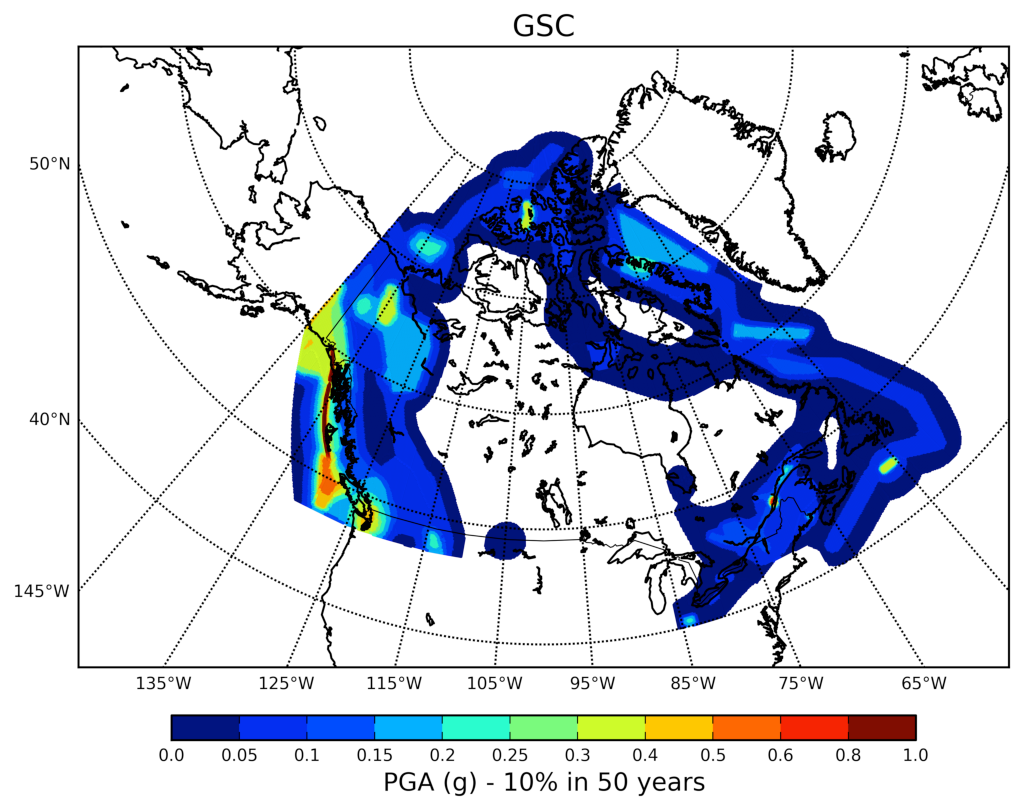
\includegraphics[width=14cm]{./qareport/pictures/GSC_combined_PGA_0pt1_firm_ground.pdf}
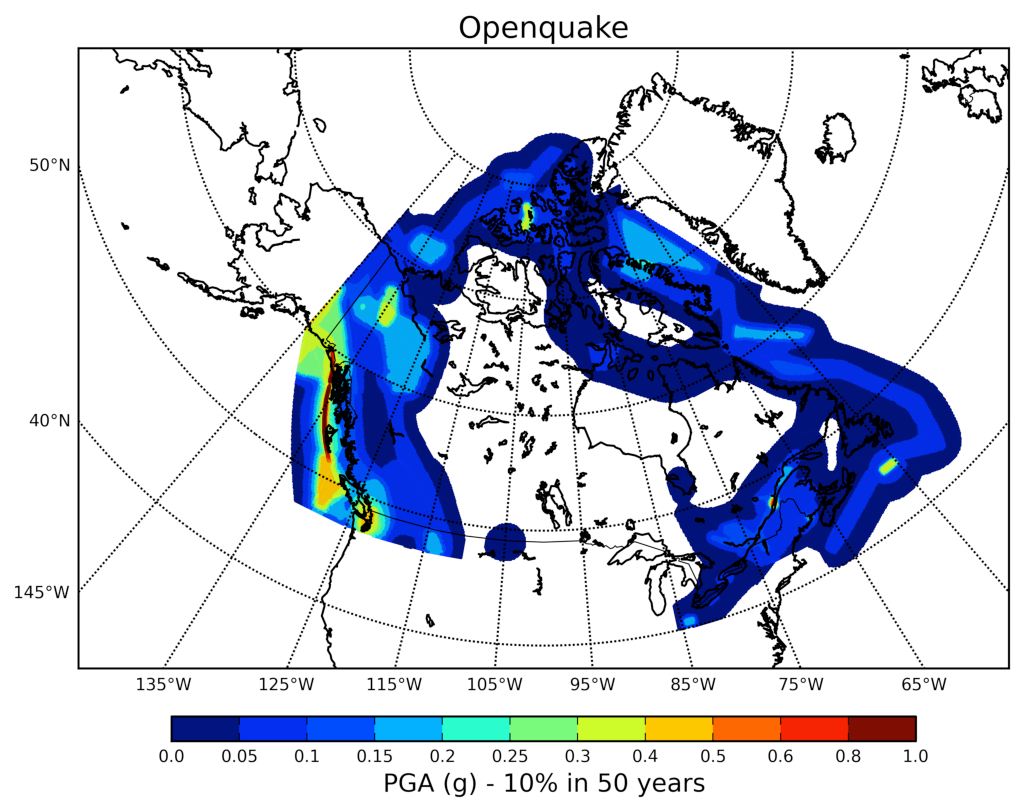
\includegraphics[width=14cm]{./qareport/pictures/OQ_combined_PGA_0pt1_firm_ground.pdf}
\caption{Official hazard map produced by the Geological Survey of Canada (top) and by the OpenQuake-engine implementation (bottom)}
\label{fig:canada_475y_hmaps}
\end{figure}
\begin{figure}
\centering
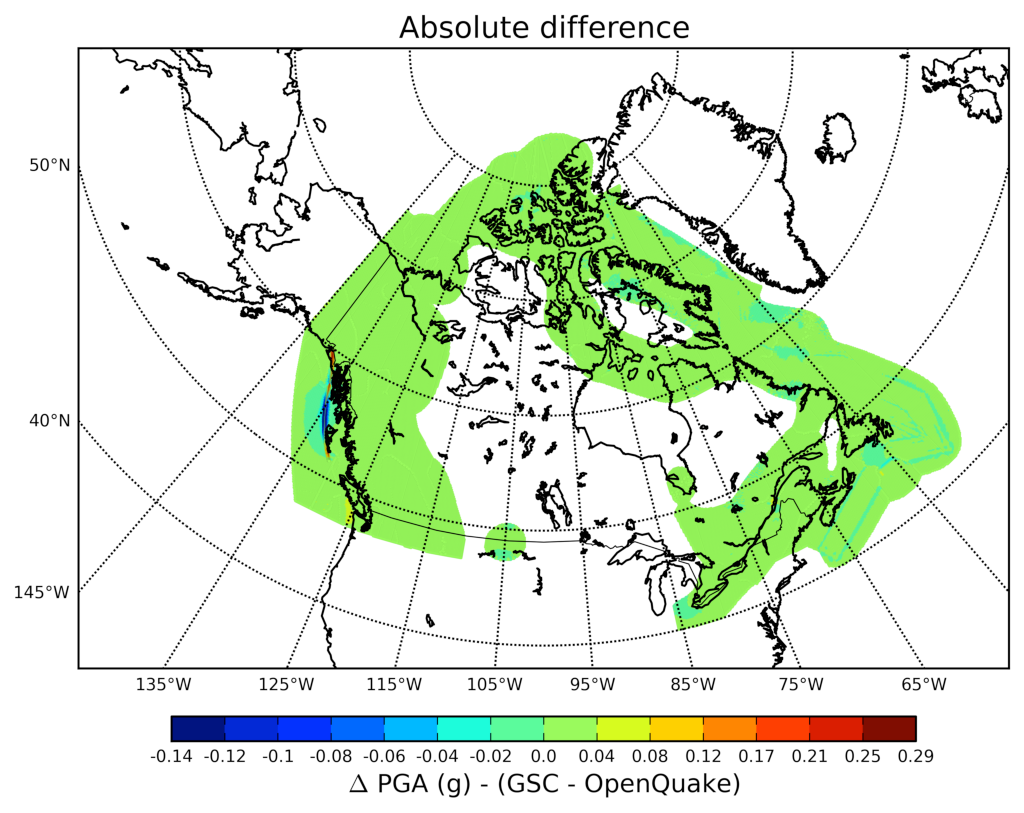
\includegraphics[width=14cm]{./qareport/pictures/GSC_OQ_PGA_0pt1_abs_diff.pdf}
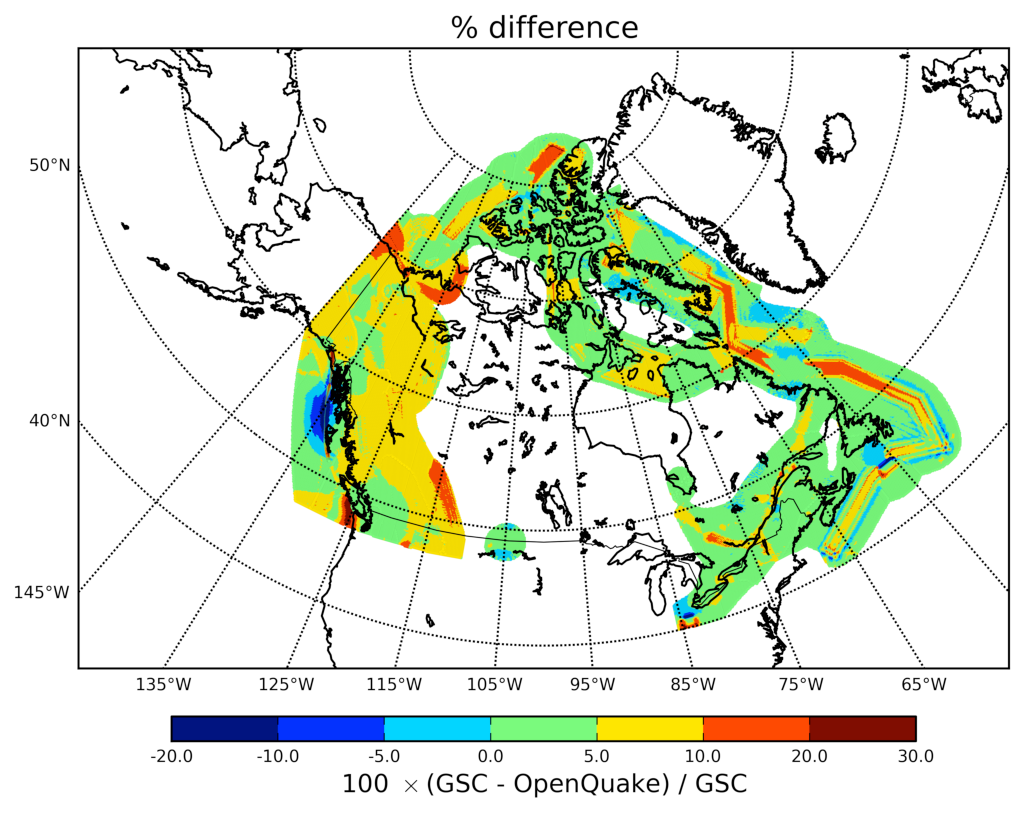
\includegraphics[width=14cm]{./qareport/pictures/GSC_OQ_PGA_0pt1_percent_diff.pdf}
\caption{Absolute (top) and percent (bottom) difference maps between the official GSC hazard map and the one produced by the OpenQuake-engine as visible in Figure \ref{fig:canada_475y_hmaps}}
\label{fig:canada_475y_dmaps}
\end{figure}
The comparison between the hazard maps reveals a satisfactory agreement, at least from a visual perspective. Difference maps (Figure \ref{fig:canada_475y_dmaps}) are however more informative and provide a quantitative understanding of the differences between the two maps. The absolute difference map shows that for the vast majority of the grid points, the GSC solution over-estimates the OpenQuake-engine solution by values between 0 and 0.04 g. The highest positive differences (GSC > OpenQuake-engine), up to 0.3 g, are instead only visible along the Queen Charlotte fault, especially at the north and south endings of the fault trace. The highest negative differences (GSC < OpenQuake-engine) are still along the Queen Charlotte fault, especially in the region close to the middle part of the fault trace. These differences can be reasonably motivated by the previously mentioned fact that, for the Queen Charlotte fault, we cannot use in the OpenQuake-engine a magnitude-length scaling relationship as originally defined by the model. We thus used the \cite{wells1994} magnitude-area scaling relationship. The discrepancies reflect not only different functional forms but also different ways of defining ruptures' size and shape. Indeed when using a magnitude-length scaling relationship, no rupture reshaping (for area conservation) is required which is instead a key feature when considering a magnitude-area scaling law. The relative percent error shows instead the significance of the absolute difference in the various regions covered by the hazard map. Percent differences ranges from $-20\%$ to $30\%$. The highest positive differences are visible along the area sources associated with low hazard values. Some significant differences are visible along the boundaries of rectangular zones such as the small rectangular area source close to the village of Anna, in Ohio, U.S. (85W, 40N) and the source south of the Newfoundland, Canada (approximately 60W, 45N). Inside those sources the hazard levels are relatively high (between 0.15 and 0.2 g for the former and between 0.3 and 0.4 for the latter). Within the boundary the relative error is less than $5\%$. The larger differences along the boundary may be therefore the effect of different discretization algorithms in the two software.


\section{The 2008 U.S. national seismic hazard model}

\subsection{The seismic source model}
To reproduce earthquake occurrences in various tectonic settings, the seismic source model defines different typologies of seismic sources: gridded-seismicity, uniform seismicity zones, and fault sources. \\
Gridded-seismicity and source zones are used to model seismicity occurring off known faults, and moderate-size earthquakes not included in fault sources. Occurrence rates are defined through a Gutenberg-Richter magnitude frequency distribution, with minimum magnitude equal to 5. Earthquakes smaller than $M=6$ are treated as point ruptures, while for larger events finite ruptures are generated. Rupture lengths are determined by using the magnitude-length scaling relationship of \cite{wells1994}. Uncertainties in rupture strike are taken into account by assigning to each site an average distance from ruptures with strike directions uniformly distributed from $0^{\circ}$ to $180^{\circ}$. Dipping ruptures are also modeled in the western U.S. by including an average hanging-wall effect.\\
For the most part, fault sources are defined to model earthquakes with magnitude larger than 6.5. Alternative fault source models are defined to take into account different magnitude-frequency distributions (Characterisitic - \cite{schwartscoppersmith1984} - and Gutenberg-Richter) and geometries.\\
The source model distinguishes between central and eastern U.S. (CEUS) and western U.S. (WUS). In CEUS the maximum magnitude is distributed between 6.6 and 7.2 for cratonic regions, and between 7.1 and 7.7 for the extended margin. Four alternative gridded-seismicity models are defined: three that take into account different completeness levels and one that considers uniform source zones for the Eastern Tennessee and New Madrid seismic zones. A number of uniform background zones are also defined to provide a hazard floor in areas with little or no historical seismicity. Fault sources are defined for the New Madrid seismic zone, and for the Meers fault (Oklahoma) and Cheraw fault (Colorado). For New Madrid, five possible fault traces are defined and three possible return periods (500-year, 750-year, 1000-year) are considered. Moreover, a temporal clustering model is also included which considers the possible occurrence of three dependent events. For the Charleston (South Carolina) seismic zone, two source zones are defined in connection with the $M=7.3$ event occurred in 1886.\\
In WUS, the maximum magnitude for gridded (shallow) seismicity is 7.0 in most regions. Exceptions include areas close to modeled faults. If a fault follows a Gutenberg-Richter magnitude frequency distribution, then the maximum magnitude in the neighbouring region is set to 6.5 (which is the $M_{min}$ of the fault Gutenberg-Richter relation). If a fault follows a Characteristic model, then the maximum magnitude is set to the minimum between 7.0 and the fault characteristic magnitude. For deep seismicity, the maximum magnitude is instead set to 7.2. For shallow seismicity, a single gridded-seismicity model is defined which, together with a number of uniform background zones and special zones, represent the overall distributed seismicity in WUS. Fault sources are defined for specific regions: the Intermountain West, Pacific Northwest (including Cascadia subduction faults), and California. Earthquake occurrence rates are both described by a Characteristic and Gutenberg-Richter distribution. Epistemic uncertainties of $\pm 0.2$ magnitude units are defined for both the Characteristic earthquake magnitude and the maximum magnitude of the Gutenberg-Richter relation. In addition to epistemic uncertainties, aleatory variability is included for characteristic earthquakes using a normal distribution with standard deviation of 0.12.

\subsection{The ground motion model}
The ground motion model specifies different sets of GMPEs for CEUS and WUS. For CEUS, a set of seven GMPEs is defined to represent the epistemic uncertainties in the ground motion modeling: \cite{frankel1996}, \cite{somerville2001}, \cite{campbell2003SCR}, \cite{toro1997}, \cite{atkinson2006}, \cite{tavakoli2005}, \cite{silva2002}. For active shallow crust in WUS, the GMPEs used are \cite{boore2008}, \cite{campbell2008}, and \cite{chiou2008}. For subduction interface events (Cascadia) the GMPE models adopted are: \cite{y1997}, \cite{ab2003}, \cite{zhao2006}. For subduction intraslab the GMPEs of \cite{geomatrix1993} and \cite{ab2003} are used instead. For active shallow crust in WUS, an additional level of epistemic uncertainties is included to take into account data limitations especially for large earthquakes. Indeed, for each GMPE, two symmetrical relationships are obtained by adding/subtracting a scaling factor to the median value.

\subsection{Reference site conditions}
Hazard maps are computed for a reference site condition corresponding to the 'NEHRP B/C site' condition which is associated to a $V_{s30}$ value equal to 760.0 m/s. The GMPEs used for active shallow crust in WUS allows for a direct usage of the $V_{s30}$ value. For subduction GMPEs the 'rock' site class is selected instead. Some of the CEUS GMPEs do not support the B/C site conditions. Therefore a 'kappa' correction is applied to convert CEUS GMPEs from hard rock to firm rock condition.

\subsection{Implementation of the model in the OpenQuake-engine}
In the OpenQuake-engine implementation, gridded-seismicity models and uniform seismicity zones are defined as collections of point sources. Point source properties reflect model's specification. If the model defines uncertain ruptures strike, then each point source is associated to multiple strike values (between $0^{\circ}$ and $180^{\circ}$ for vertical ruptures and between $0^{\circ}$ and $360^{\circ}$ for dipping ruptures) otherwise a single strike is defined. For 'shallow' gridded seismicity models, the hypocentral depth is set to 7.5 km (equal to the depth of the centroid of dipping rupture planes (\cite{petersen2008})) and the lower seismogenic depth is set to 15 km. Deep seismicity is assumed to occur at an hypocentral depth of 50 km, and the seismogenic layer is assumed to extend between 50 and 100 km. Crustal faults are defined as simple fault sources (with discretization step of 4 km), while Cascadia subduction interface faults are defined as complex fault sources (with discretization stepf of 10 km). The magnitude-area scaling relationship of \cite{wells1994} is used for all models (gridded-seismicity and fault based) both in WUS and CEUS. In the current OQ-engine implementation, all source models are included except the cluster model for the New Madrid seismic zone (only the unclustered source model is considered). To combine models from different logic tree branches, we compute for each source a magnitude-frequency distribution whose occurrence rates are scaled by the branch weight. For each site, contributions coming from ruptures that are within 1000 km are considered for the CEUS and Cascadia models, and 200 km for the gridded-seismicity and the shallow crustal faults models in WUS. Ground motion distribution is truncated at three sigmas (\cite{petersen2008}). Epistemic uncertainties on GMPE median values for WUS active shallow crust are not yet implemented.

\begin{figure}
\centering
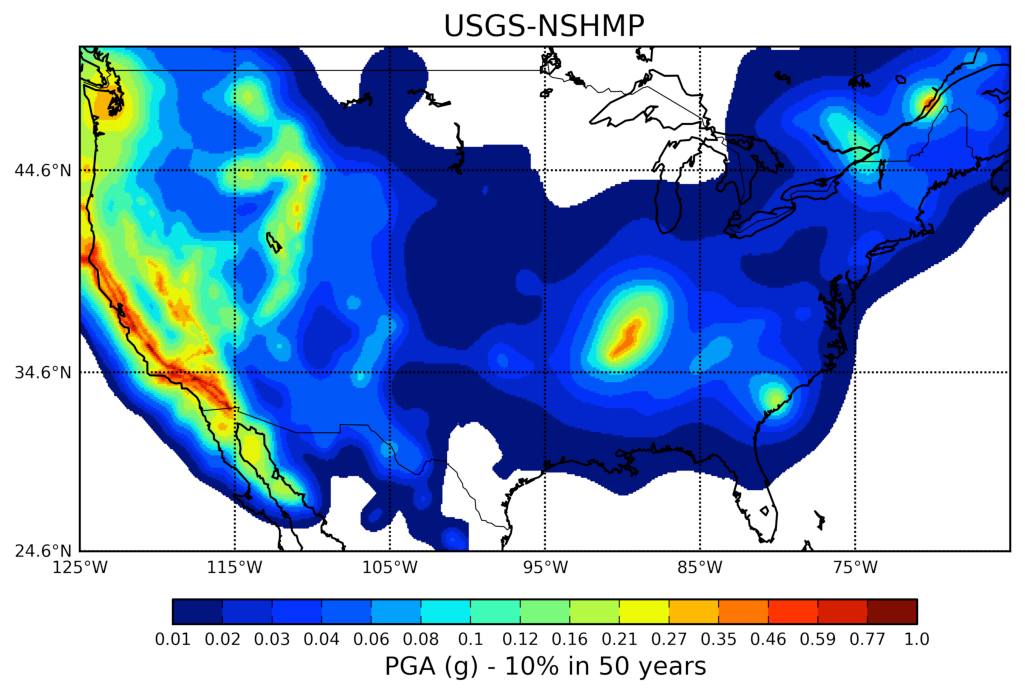
\includegraphics[width=14cm]{./qareport/pictures/map_usa_PGA_0pt1_NSHMP.pdf}
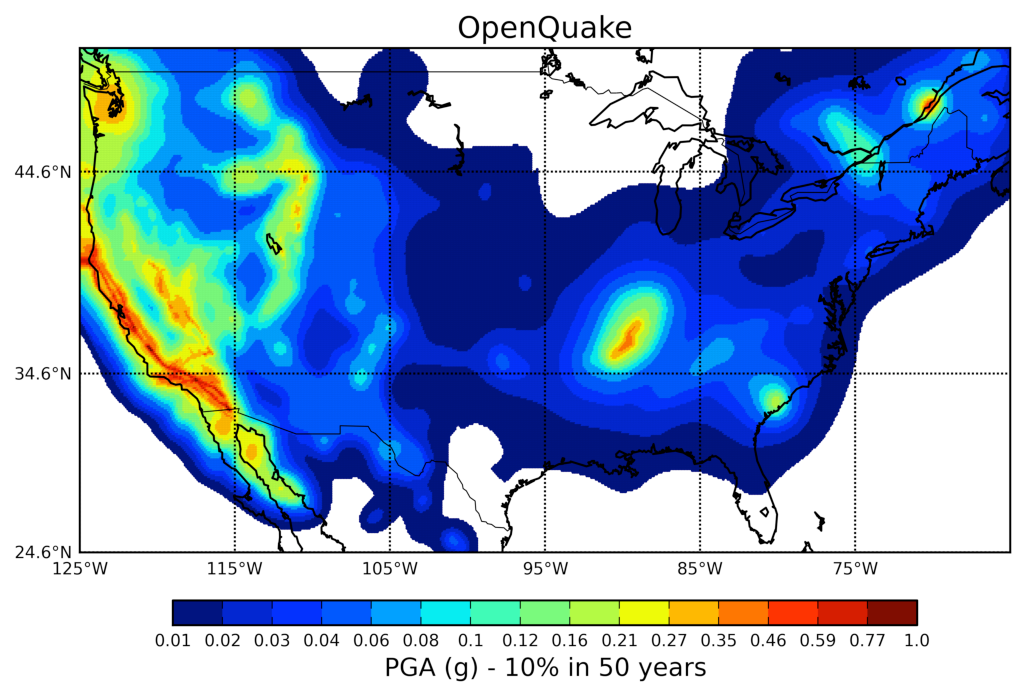
\includegraphics[width=14cm]{./qareport/pictures/map_usa_PGA_0pt1_OQ.pdf}
\caption{Official hazard map produced by the USGS-NSHMP (top) and by the OpenQuake-engine implementation (bottom)}
\label{fig:usa_475y_hmaps}
\end{figure}
\begin{figure}
\centering
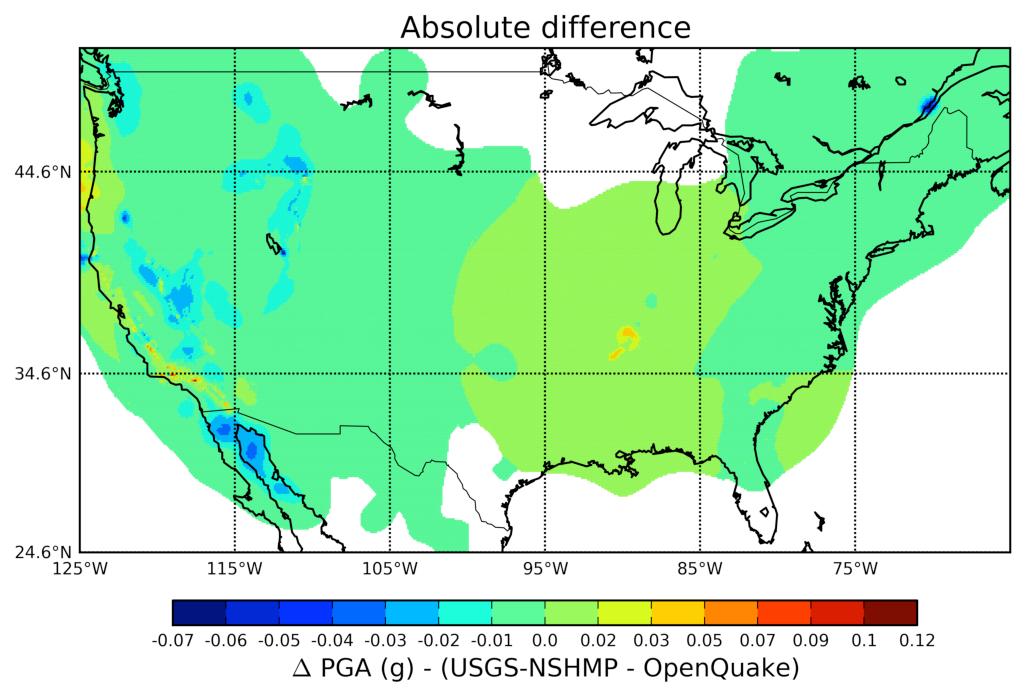
\includegraphics[width=14cm]{./qareport/pictures/map_usa_PGA_0pt1_abs_diff_NSHMP_OQ.pdf}
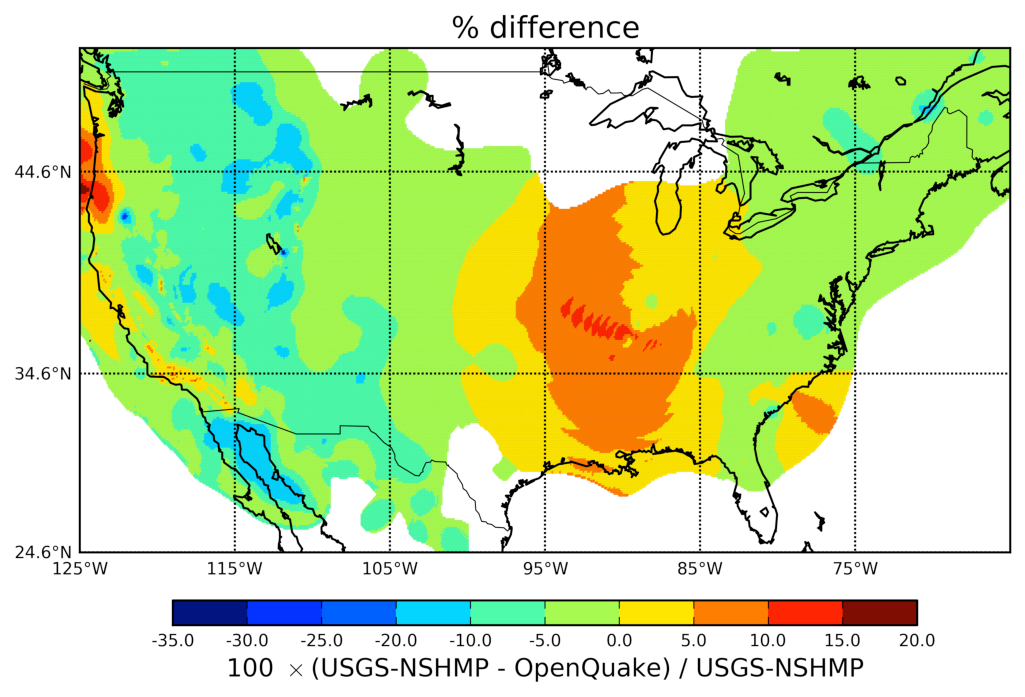
\includegraphics[width=14cm]{./qareport/pictures/map_usa_PGA_0pt1_percent_diff_NSHMP_OQ.pdf}
\caption{Absolute (top) and percent (bottom) difference maps between the official USGS-NSHMP hazard map and the one produced by the OpenQuake-engine as visible in Figure \ref{fig:usa_475y_hmaps}}
\label{fig:usa_475y_dmaps}
\end{figure}

\subsection{Comparison against USA hazard map}
The comparison between PGA hazard maps for $10\%$ probability of exceedance in 50 years produced by the USGS-NSHMP and by the OpenQuake-implementation is shown in Figure \ref{fig:usa_475y_hmaps}. The visual comparison shows an overall agreement. A more quantitative view on the differences between the two maps is given in Figure \ref{fig:usa_475y_dmaps}. Absolute differences range from -0.07 g to 0.12 g. For the vast majority of the sites, differences range from -0.01 g 0.02 g. Close to WUS crustal faults (except California) and in the Charlevoix (Quebec, Canada) zone the OQ-engine provides larger values. On the contrary, close to some southern California crustal faults and close to the New Madrid zone the OQ-engine provides lower values than the USGS-NSHMP. This is also visible in the percent difference map, where in a broad area around the New Madrid seismic zone differences range mostly from $0$ to $10\%$ with peak values up to $15\%$. Lower values in the OpenQuake-engine solutions are also visible close to the Charleston zone and in Oregon/Washington states (WUS).\\
Differences in the New Madrid zone can be accounted for by the absence, in the OQ-engine implementation, of the clustered source model. Discrepancies in the WUS can be instead explained as due to the missing epistemic uncertainties in the GMPE median value for shallow crustal sources. In addition to that, differences can arise because of the different scaling relationship used. In California, the model of \cite{hanks2002} is used, while in the OpenQuake-engine calculation the model of \cite{wells1994} is adopted.